\chapter{Pruebas}\label{cap:pruebas}

\section{Introducción}

En este capítulo se van a describir las pruebas realizadas a la aplicación desarrollada, para asegurar que su funcionamiento es el correcto, amigable y robusto, es decir, puede recuperarse de los errores que puedan ocurrir durante su utilización.

Debido a que esta es una versión actualizada de una anterior, las pruebas irán principalmente enfocadas a aquellas funcionalidades que contenían algún error o aquellas que sean nuevas. Además, gracias a la división del programa en módulos, se podrán clasificar las pruebas de forma más sencilla.

Dada la división modular de la aplicación, las pruebas se han agrupado por los módulos que la componen:

\begin{itemize}
  \item \textbf{Módulo Editor}.
  \item \textbf{Módulo Simulador}.
\end{itemize}

Finalmente, para cada prueba realizada, se detallará el objetivo de la prueba, el proceso llevado a cabo, el resultado de la misma y la acción tomada (en caso de haber detectado e\-rrores en el software).

\section{Pruebas del módulo Editor}

En esta sección se recopilan todas las pruebas efectuadas al módulo de Edición de gramáticas.


\subsection{Persistencia en la modificación de gramáticas}

\textbf{Objetivo}: comprobar que la creación y modificación de gramáticas persiste correctamente en el sistema, evitando la pérdida de datos observada en algunas ocasiones en SimAS 2.0.
\medskip

\textbf{Proceso}: se partió de una gramática existente y se realizaron modificaciones sobre sus elementos (terminales, no terminales y producciones). A continuación, se guardó la gramática y se volvió a abrir para verificar que todos los cambios se conservaban. En las figuras se ilustran los pasos clave del proceso:
\medskip

\needspace{6cm}
\begin{figure}[H]
  \centering
  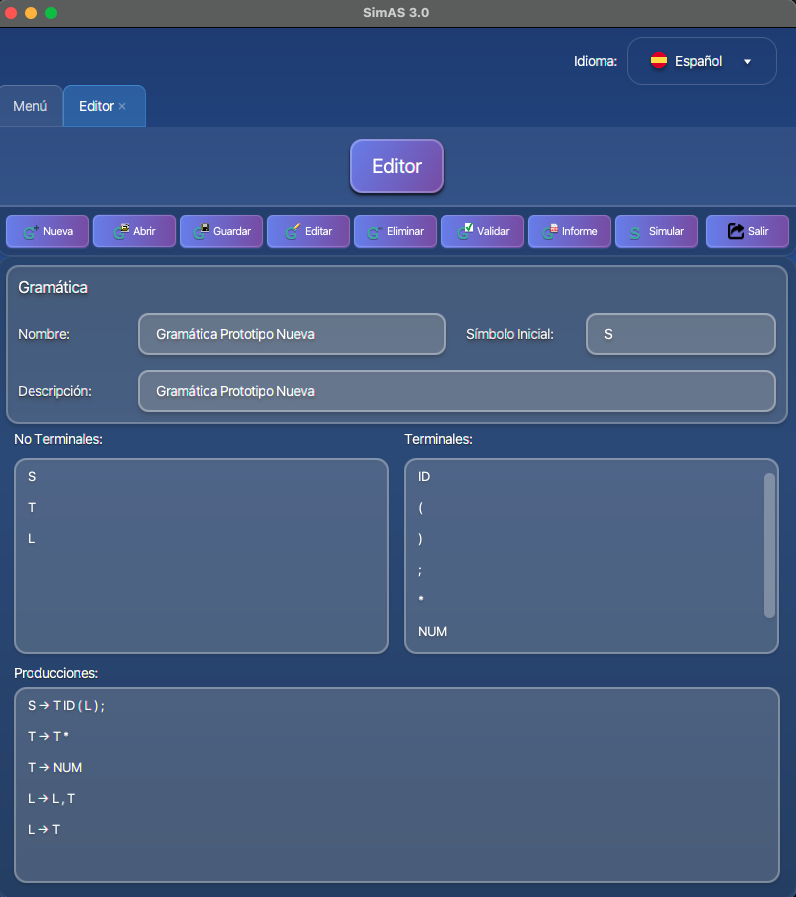
\includegraphics[width=0.75\textwidth]{figuras2/pruebas/editor/gramatica_original.png}
  \caption{Gramática original cargada en el editor.}
\end{figure}

\needspace{6cm}
\begin{figure}[H]
  \centering
  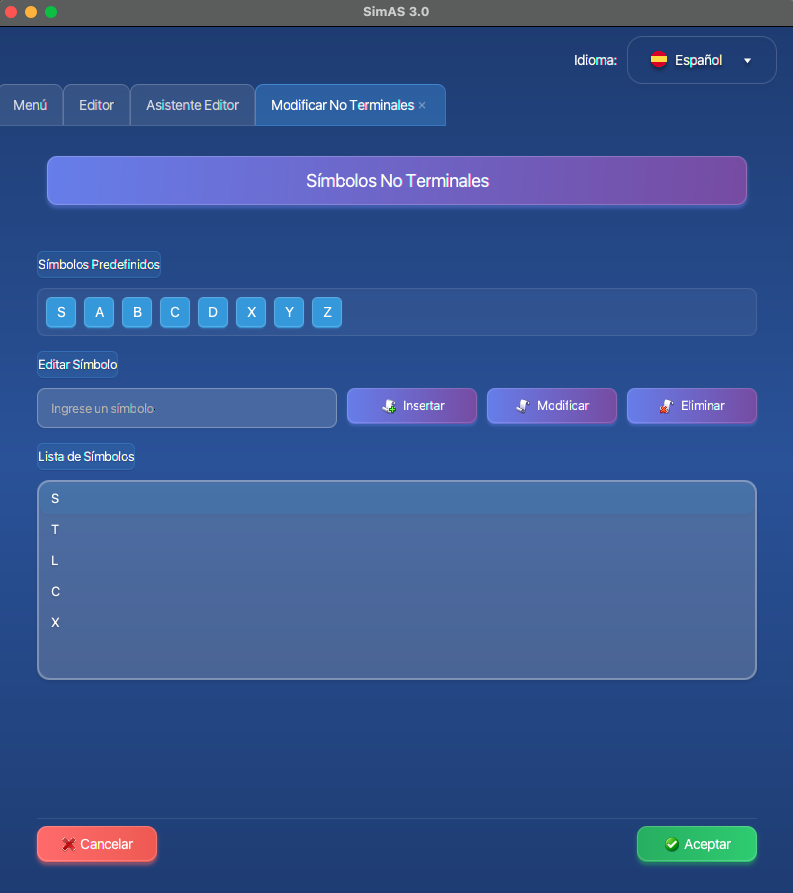
\includegraphics[width=0.75\textwidth]{figuras2/pruebas/editor/nuevos_terminales.png}
  \caption{Edición y adición de terminales.}
\end{figure}

\needspace{6cm}
\begin{figure}[H]
  \centering
  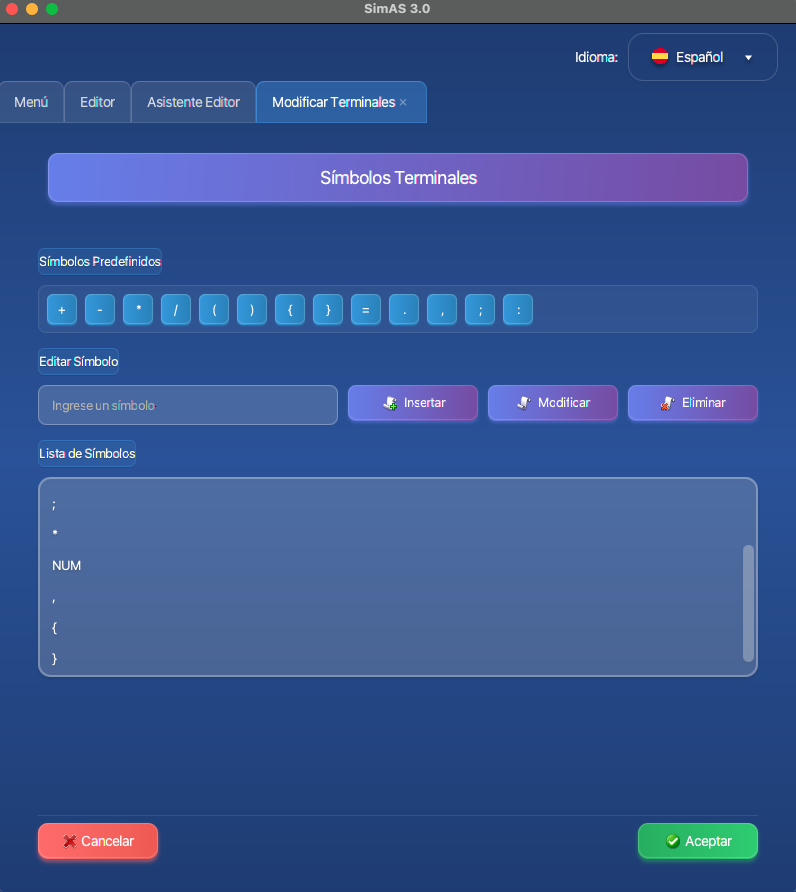
\includegraphics[width=0.75\textwidth]{figuras2/pruebas/editor/nuevos_no_term.png}
  \caption{Edición y adición de no terminales.}
\end{figure}

\needspace{6cm}
\begin{figure}[H]
  \centering
  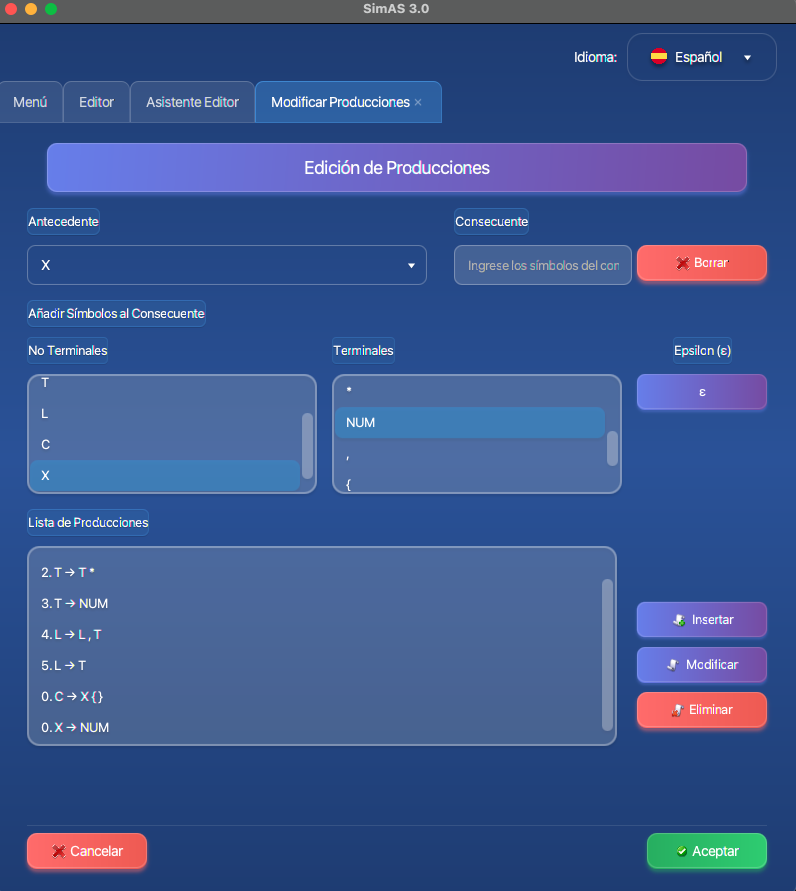
\includegraphics[width=0.75\textwidth]{figuras2/pruebas/editor/nuevas_prod.png}
  \caption{Edición y adición de producciones.}
\end{figure}

\needspace{6cm}
\begin{figure}[H]
  \centering
  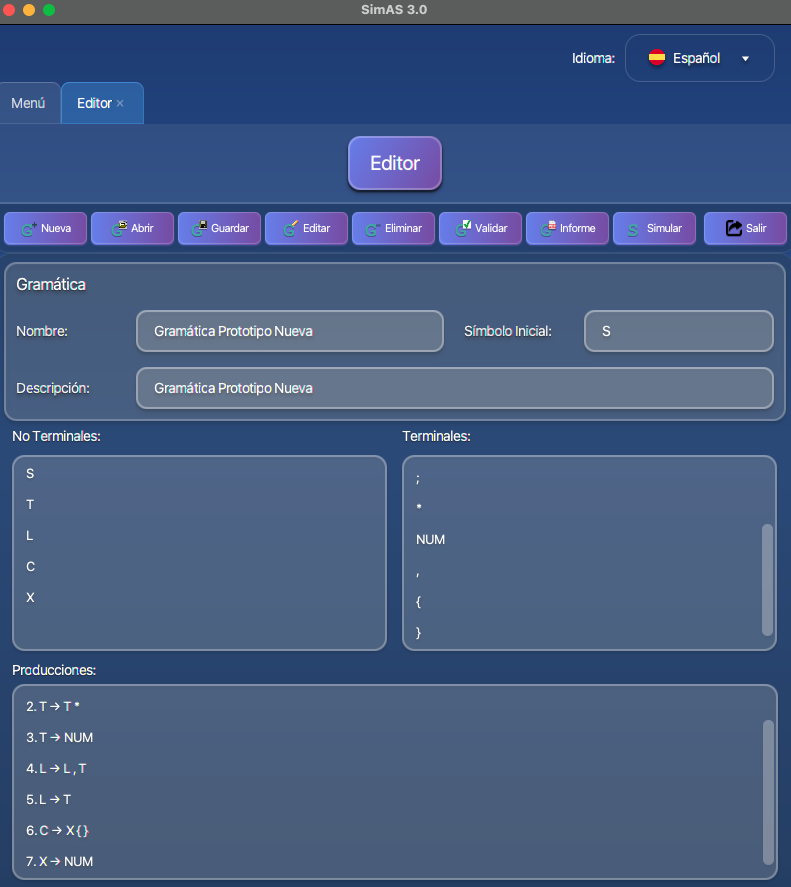
\includegraphics[width=0.75\textwidth]{figuras2/pruebas/editor/gramatica_nueva.png}
  \caption{Gramática guardada y recargada con los cambios persistidos.}
\end{figure}

\textbf{Resultado}: tras cerrar y volver a abrir la gramática, todos los cambios se mantuvieron correctamente. No se reprodujo la pérdida de datos reportada en SimAS 2.0.
\medskip

\textbf{Solución adoptada}: se revisó y corrigió la capa de persistencia para asegurar un guardado atómico de la gramática y una serialización consistente de todos sus componentes (terminales, no terminales, producciones y metadatos), además de sincronizar el modelo con la vista previamente al guardado. Con ello, el problema quedó resuelto.

\subsection{Complejidad al añadir producciones}

\textbf{Objetivo}: simplificar y hacer más intuitivo el proceso de añadir producciones en el editor, reduciendo la complejidad que presentaba SimAS 2.0 y mejorando la experiencia de uso.
\medskip

\textbf{Proceso}: se partió de una gramática existente y se procedió a añadir nuevas producciones mediante el panel de modificación. Las nuevas producciones se agregan inicialmente con ID=0 en la lista de producciones, permitiendo al usuario editarlas antes de confirmar. Al hacer clic en "Aceptar", el sistema asigna automáticamente los IDs correspondientes de forma secuencial. En las figuras se muestra el proceso paso a paso:
\medskip

\needspace{6cm}
\begin{figure}[H]
  \centering
  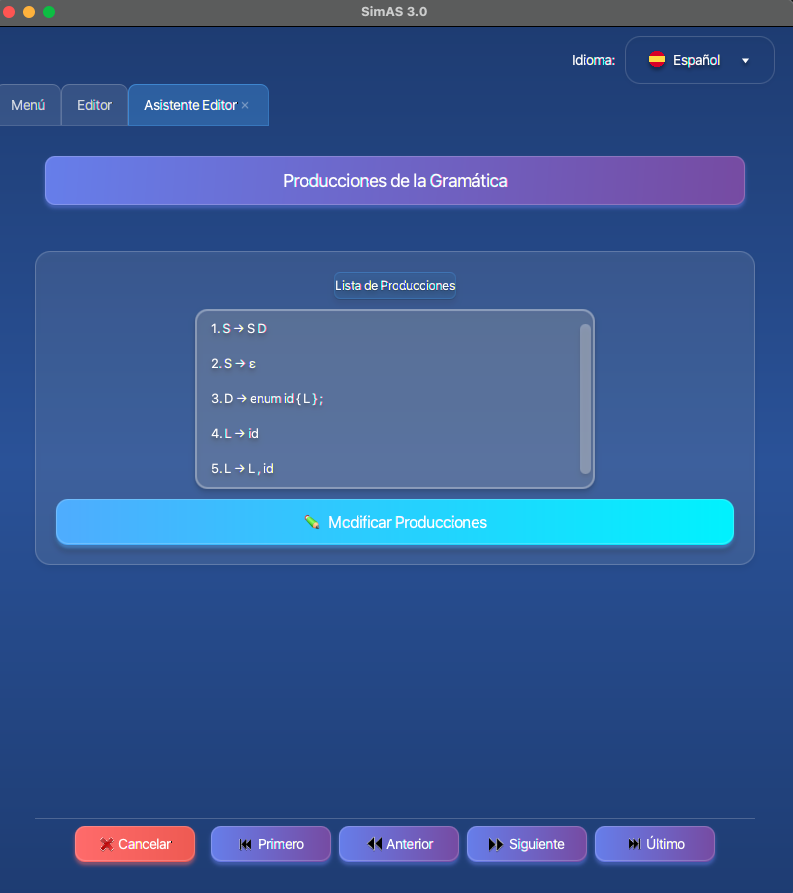
\includegraphics[width=0.75\textwidth]{figuras2/pruebas/editor/old_prod.png}
  \caption{Lista de producciones original antes de añadir nuevas.}
\end{figure}

\needspace{6cm}
\begin{figure}[H]
  \centering
  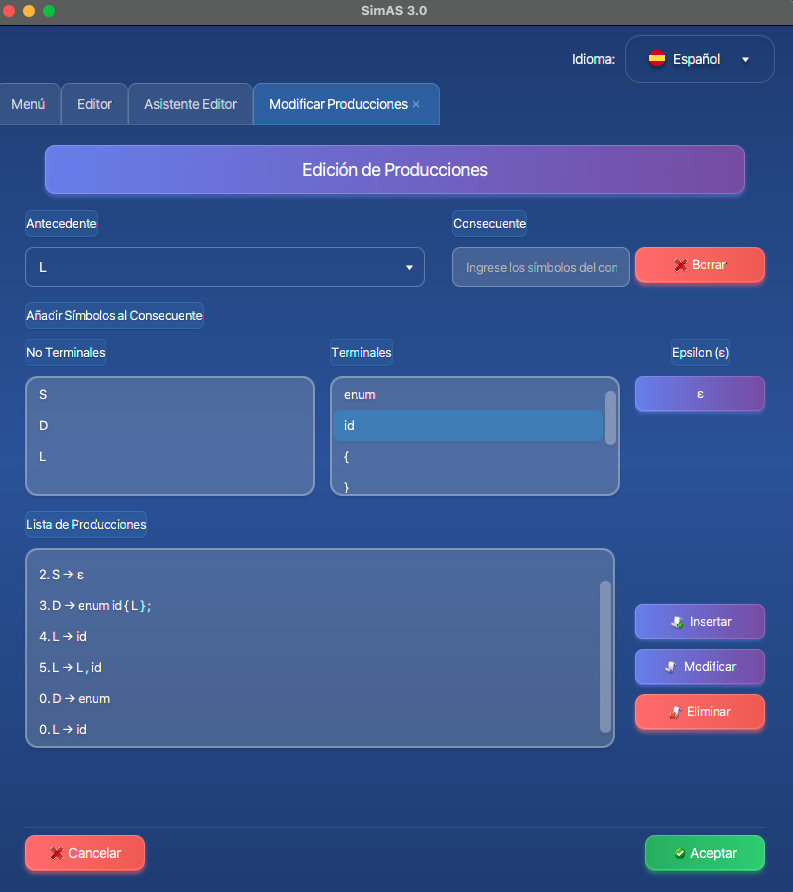
\includegraphics[width=0.75\textwidth]{figuras2/pruebas/editor/mod_prod.png}
  \caption{Añadiendo nuevas producciones con ID=0 temporal.}
\end{figure}

\needspace{6cm}
\begin{figure}[H]
  \centering
  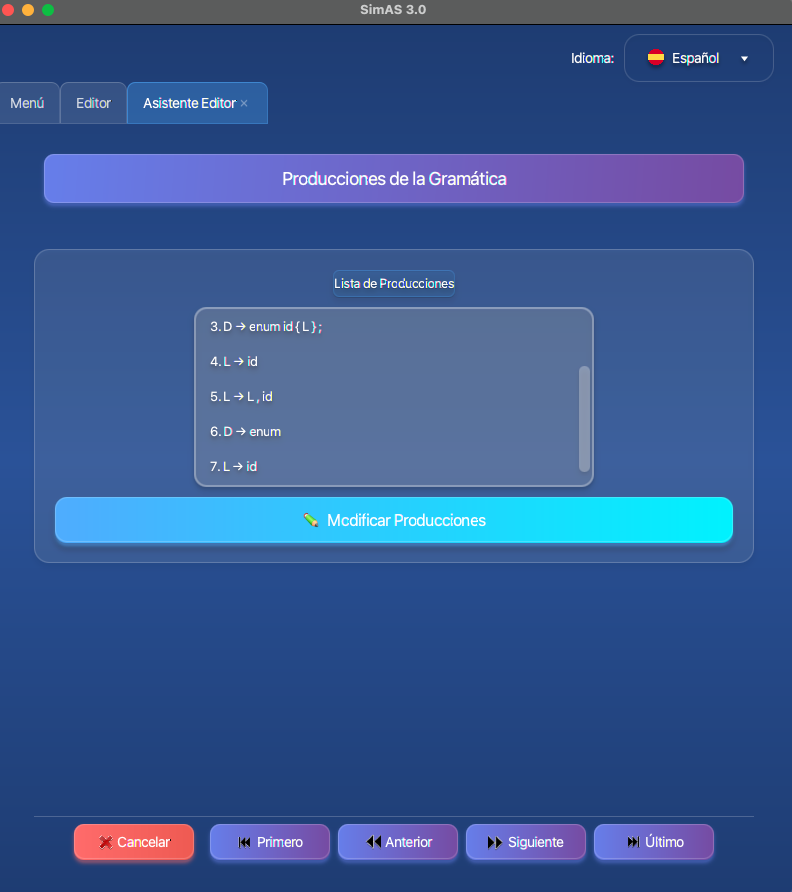
\includegraphics[width=0.75\textwidth]{figuras2/pruebas/editor/new_prod.png}
  \caption{Producciones añadidas con IDs asignados automáticamente.}
\end{figure}

\textbf{Resultado}: el proceso de añadir producciones resultó mucho más intuitivo y consistente, eliminando los pasos innecesarios y reduciendo el tiempo requerido. No se detectaron errores en la asignación de IDs ni en la integración con la gramática existente.
\medskip

\textbf{Solución adoptada}: se simplificó el flujo de trabajo unificando la adición de producciones en un único panel con asignación automática de IDs. Se implementó validación inmediata de formato y símbolos, y se agregó retroalimentación visual durante el proceso para guiar al usuario. Esto garantiza una experiencia más fluida y consistente con el resto de operaciones del editor.


\section{Pruebas del módulo Simulador}

En esta sección se recopilan todas las pruebas efectuadas al módulo de Simulación de gramáticas.

\subsection{Error ocasional en la generación de conjuntos Primero y Siguiente}

\textbf{Objetivo}: verificar que la generación de los conjuntos Primero y Siguiente se realiza correctamente sin errores intermitentes, como se observaba en ocasiones en SimAS 2.0.
\medskip

\textbf{Proceso}: se cargaron diversas gramáticas en el simulador y se procedió a generar los conjuntos Primero y Siguiente. Se verificó que el proceso se completara sin fallos y que los resultados fueran consistentes en múltiples ejecuciones. A continuación se muestran ejemplos del proceso:
\medskip

\needspace{6cm}
\begin{figure}[H]
  \centering
  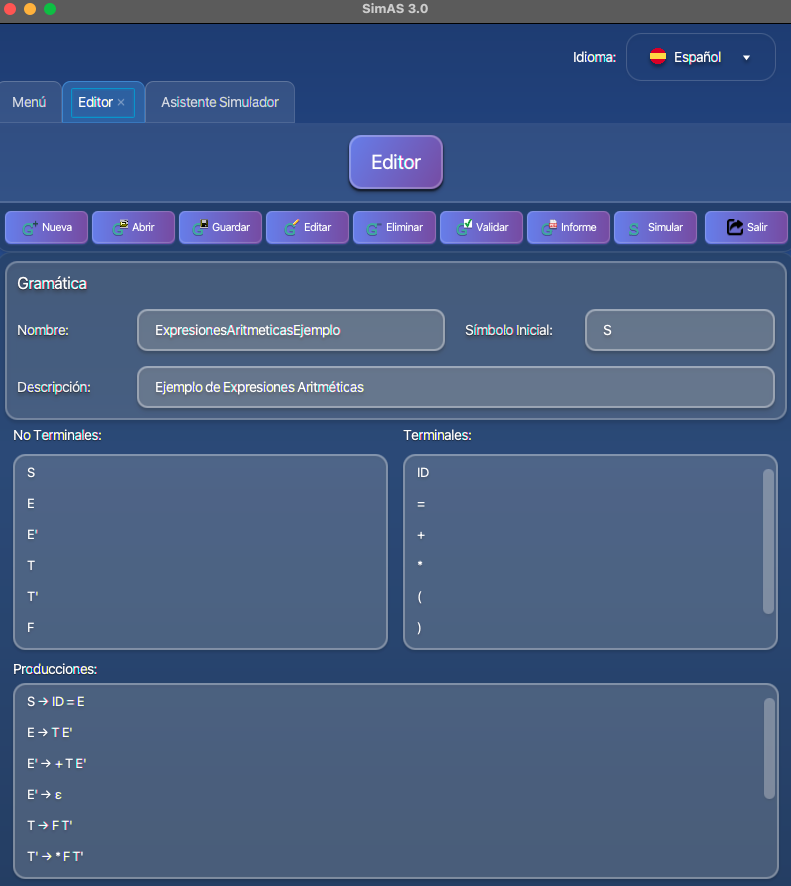
\includegraphics[width=0.75\textwidth]{figuras2/pruebas/simulador/gramatica.png}
  \caption{Gramática original cargada en el simulador.}
\end{figure}

\needspace{6cm}
\begin{figure}[H]
  \centering
  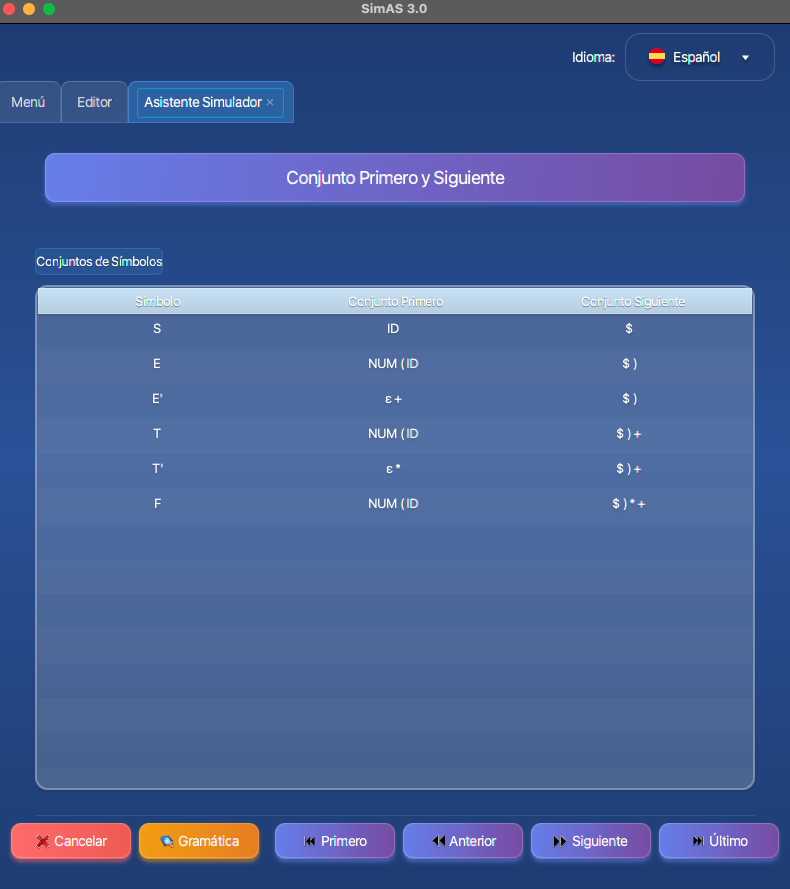
\includegraphics[width=0.75\textwidth]{figuras2/pruebas/simulador/conjuntos.png}
  \caption{Conjuntos Primero y Siguiente generados correctamente.}
\end{figure}

\textbf{Resultado}: los conjuntos Primero y Siguiente se generaron de forma correcta y consistente en todas las pruebas realizadas. No se reprodujeron los errores intermitentes observados en la versión anterior.
\medskip

\textbf{Solución adoptada}: se revisaron y corrigieron los métodos encargados de calcular los conjuntos Primero y Siguiente, asegurando un manejo adecuado de casos recursivos, reglas épsilon y dependencias entre símbolos. Se implementaron verificaciones adicionales para detectar y corregir inconsistencias durante el cálculo, garantizando resultados precisos y libres de errores.

\subsection{Problemas al añadir errores}

\textbf{Objetivo}: verificar que la inserción de errores en la tabla predictiva se realiza correctamente, resolviendo los problemas observados en SimAS 2.0 donde no se permitía la inserción en ciertas partes de la tabla.
\medskip

\textbf{Proceso}: se cargó la gramática en el simulador y se avanzó al paso 5 del asistente, donde se interactúa con la tabla predictiva completa. Se probó la nueva funcionalidad para insertar, modificar y eliminar celdas de error de forma intuitiva. A continuación se muestran los elementos clave del proceso:
\medskip

\needspace{6cm}
\begin{figure}[H]
  \centering
  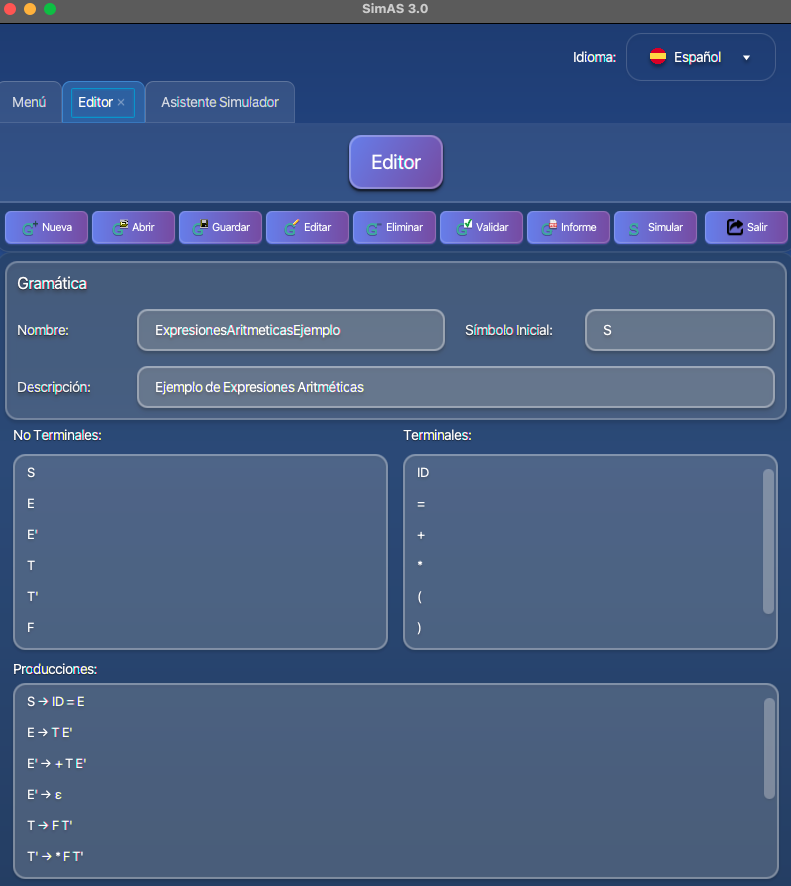
\includegraphics[width=0.75\textwidth]{figuras2/pruebas/simulador/gramatica.png}
  \caption{Gramática original utilizada para la prueba.}
\end{figure}

\needspace{6cm}
\begin{figure}[H]
  \centering
  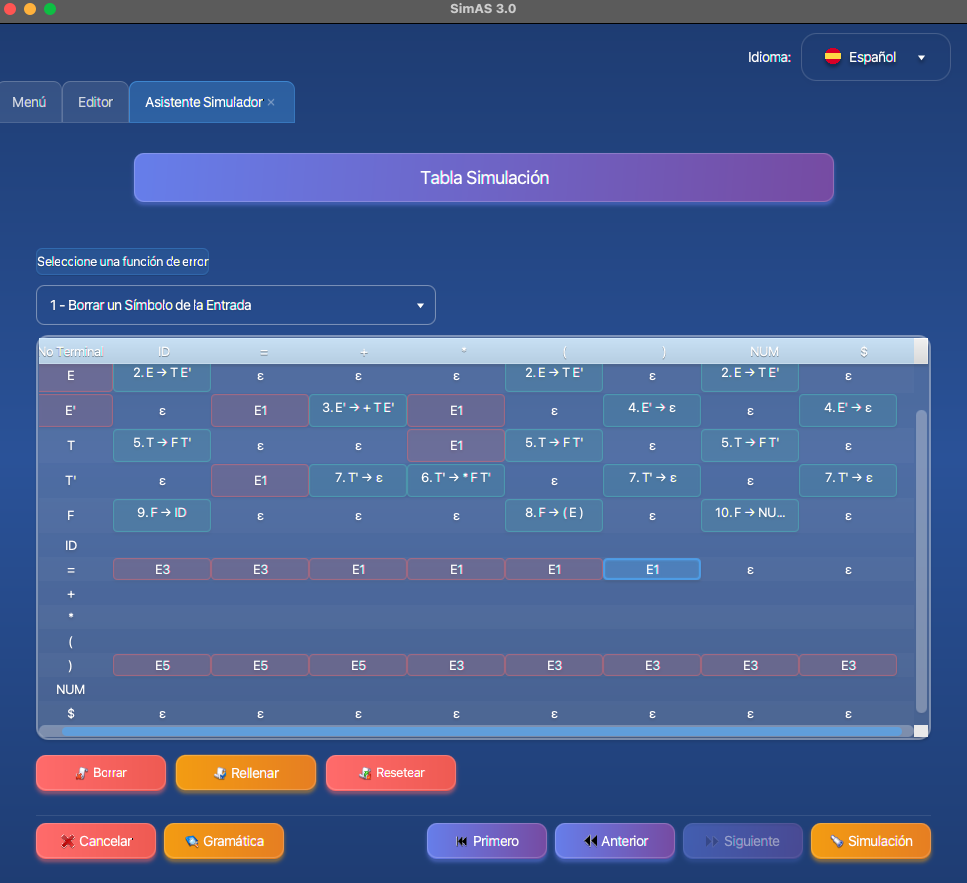
\includegraphics[width=0.75\textwidth]{figuras2/pruebas/simulador/func_errores.png}
  \caption{Nueva interfaz para gestionar funciones de error en el paso 5.}
\end{figure}

\textbf{Resultado}: la inserción, modificación y eliminación de errores en la tabla se realizó correctamente sin problemas. La nueva interfaz permite una interacción fluida con cualquier celda de la tabla, incluyendo las partes inferiores que anteriormente presentaban dificultades.
\medskip

\textbf{Solución adoptada}: se desarrolló una nueva forma de interactuar con la tabla en el paso 5 del asistente de simulador, implementando controles intuitivos para inserción, modificación y eliminación de celdas. Se agregó validación en tiempo real y retroalimentación visual para guiar al usuario durante el proceso, garantizando que los errores sintácticos puedan simularse y corregirse de manera efectiva.

\subsection{Generación parcial de árboles de análisis}

\textbf{Objetivo}: verificar que la generación completa de árboles sintácticos se realiza correctamente, incluyendo nodos con el símbolo épsilon, resolviendo las limitaciones observadas en SimAS 2.0.
\medskip

\textbf{Proceso}: se cargó una gramática en el simulador y se inició el proceso de simulación con una cadena de entrada específica. Se observó cómo el nuevo método robusto construye el árbol de análisis de manera progresiva, mostrando su evolución en tiempo real durante la simulación. A continuación se ilustran los elementos clave:
\medskip

\needspace{6cm}
\begin{figure}[H]
  \centering
  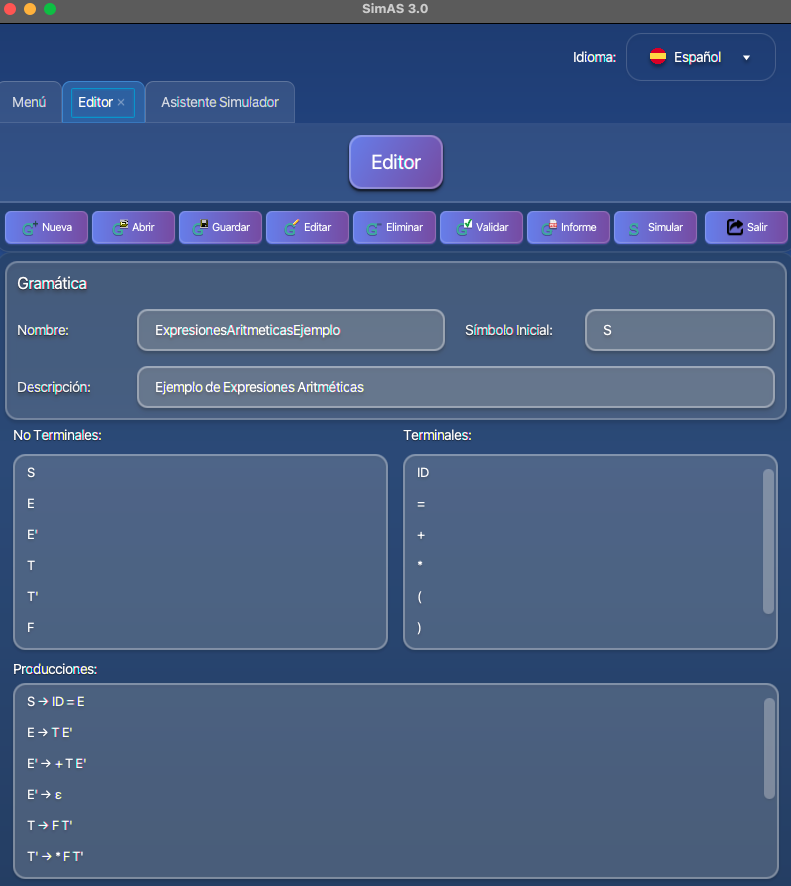
\includegraphics[width=0.75\textwidth]{figuras2/pruebas/simulador/gramatica.png}
  \caption{Gramática original utilizada para la prueba.}
\end{figure}

\needspace{6cm}
\begin{figure}[H]
  \centering
  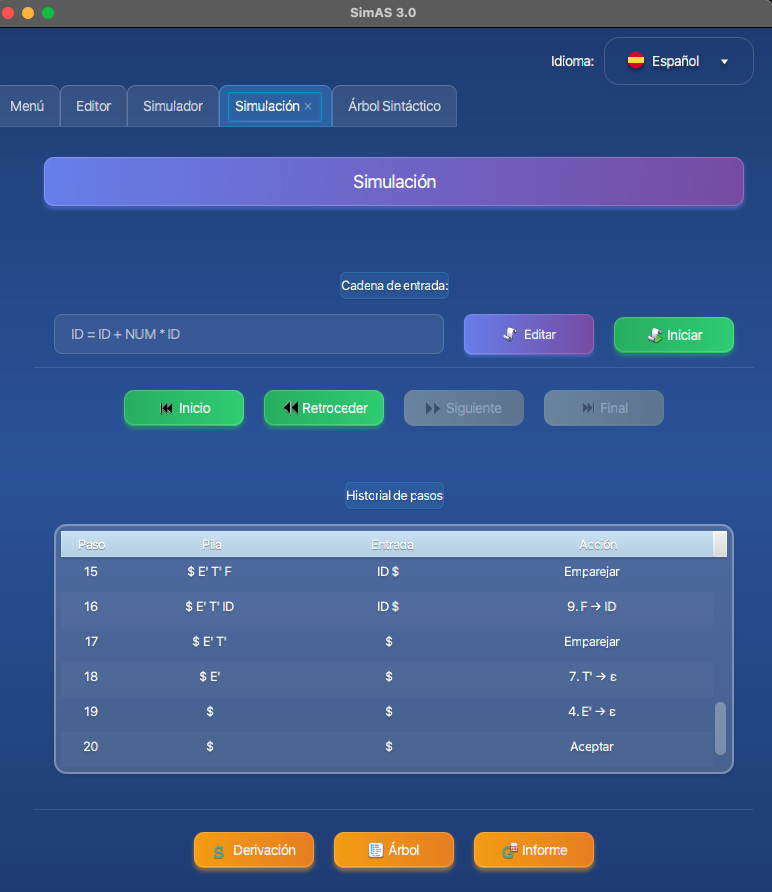
\includegraphics[width=0.7\textwidth]{figuras2/pruebas/simulador/cadena_entrada.png}
  \caption{Cadena de entrada utilizada para la simulación.}
\end{figure}

\needspace{6cm}
\begin{figure}[H]
  \centering
  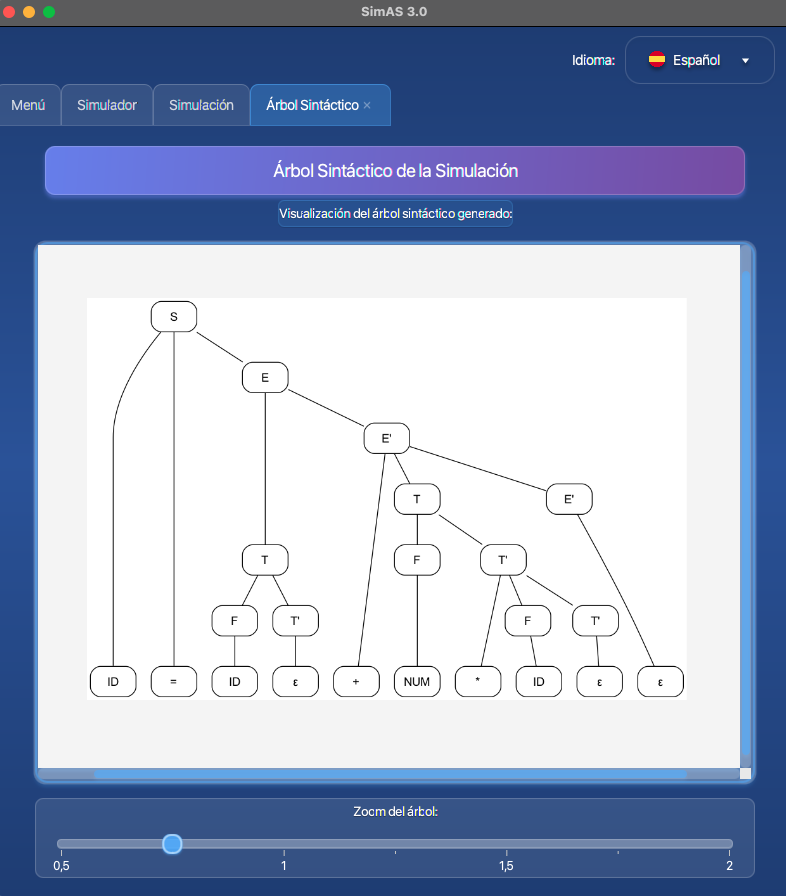
\includegraphics[width=0.7\textwidth]{figuras2/pruebas/simulador/arbol.png}
  \caption{Árbol sintáctico generado completamente durante la simulación.}
\end{figure}

\textbf{Resultado}: el árbol de análisis se generó de forma completa y correcta, incluyendo correctamente los nodos con el símbolo épsilon. El proceso de construcción progresiva permite visualizar la evolución del árbol en tiempo real, facilitando la comprensión del análisis sintáctico.
\medskip

\textbf{Solución adoptada}: se construyó un método robusto para la generación de árboles durante el proceso de simulación, implementando algoritmos específicos para manejar correctamente el símbolo épsilon y otros casos especiales. Se agregó funcionalidad para mostrar el árbol de manera progresiva conforme avanza la simulación, proporcionando una experiencia visual intuitiva para el usuario.

\subsection{Limitación en la generación de informes}

\textbf{Objetivo}: verificar que la funcionalidad de generación de informes se realiza correctamente, resolviendo las limitaciones significativas observadas en versiones anteriores.
\medskip

\textbf{Proceso}: se probaron las tres modalidades de informes disponibles (editor, simulador y simulación) para confirmar su correcta generación. Se verificó que el informe del editor esté englobado en el del simulador, y que estos dos estén integrados en el informe de simulación completa. Además, se comprobó el sistema de nomenclatura automática para guardar los informes, que utiliza el nombre del archivo XML cargado como base.
\medskip

\textbf{Resultado}: los tres informes se generan correctamente con toda la información necesaria. La estructura jerárquica permite una navegación intuitiva desde el informe más general (simulación) hacia los más específicos (simulador y editor). Los archivos se guardan con nomenclatura automática: el informe del editor mantiene el nombre del XML original, mientras que los informes del simulador y simulación añaden "\_simulador" o "\_simulación" (según el idioma de la aplicación) al nombre base, o permiten al usuario elegir un nombre personalizado.
\medskip

\textbf{Solución adoptada}: se implementó un sistema completo de generación de informes que produce tres tipos diferenciados con estructura jerárquica. Se agregó funcionalidad de nomenclatura automática inteligente que respeta el idioma de la aplicación y permite personalización por parte del usuario, facilitando la organización y identificación de los documentos generados.

